\iflanguage{ngerman}
{\chapter{Verwandte Arbeiten}}
{\chapter{Related Work}}
\label{sec:related}

% Describing the research field with relevant works on the same or similar issues.

% Aufzeigen, wer sich bereits mit dem Thema oder ähnlichen verwandten
% Themen auseinandergesetzt hat, welche Lösungswege beschrieben wurden und was die Verbindung der jeweiligen zur eigenen Arbeit ist.
% Kurzen ausblick auf die eigene Arbeit und was man neu gemacht hat. Own Contributions


Occlusion avoidance is a well-studied area of computer visualization that is constantly evolving as technology advances.
Innovative ways to expand and enhance existing concepts and techniques are made possible by new devices and technologies. 
This is especially true for visualization methods like cutting planes and exploded views, which greatly profit from these novel interaction possibilities.
\begin{wrapfigure}{R}{0.45\textwidth}
	\centering
	\vspace{-0.8cm}
	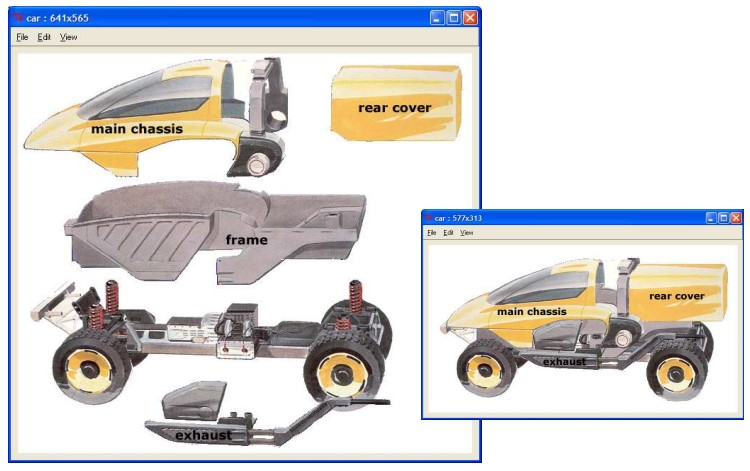
\includegraphics[width=1\linewidth]{fig/Images/Li_ExplodedView_GI04_fig16}
	\caption[]{Interactive car diagram in its fully expanded (left) and fully collapsed configurations (right). [\cite{li2004interactive}, Figure 16]}
	\vspace{-1cm}
\end{wrapfigure}

Li et al. provide an example of this.\cite{li2004interactive} In their work, they demonstrate an algorithm that automatically separates traditional drawn explosion views to make them interactive.
Their algorithm takes 2D images of explosion view diagrams and automatically cuts them apart, both reducing visual clutter and clarifying the spatial separation of the individual components. 
Furthermore, the separated parts can be labeled more precisely and retracted and extended as needed.

Since the interaction capabilities of two-dimensional images are limited and data sets and models have become increasingly complex, the question arises as to how the same principles of exploded views can be applied to three-dimensional objects.
For this purpose, Mohammad et al. developed a tool that creates exploded views for three-dimensional CAD models. It shows both precise spatial relationships and the order in which the object was assembled.\cite{Mohammad_1993}
This is especially useful when visualizing machines and technical objects, as it gives the viewer a clear idea of how the parts are arranged.
One disadvantage of their implementation is that the individual relations must be clearly defined by a designer beforehand in order to generate the explosion view and calculate the position of the exploded parts.
As a result, the order of composition and the blocking elements must be known and manually defined.

Li et al. therefore presented a system that automatically extracts non-blocking exploded views from a 3D model, focusing on rearranging parts instead of hiding obscuring geometry.\cite{Wilmot_Li_2008}
They also provide a list of tools to interact with the exploded views and dynamically select and show parts of interest.
Their implementation works for both hierarchical and non-hierarchical models, which also allows it to process biological datasets where there is no fixed assembly order.
\begin{figure}
	\centering
	\normalsize
	\begin{subfigure}[t]{0.49\textwidth}
		\centering
		%\vspace{-0.7cm}
		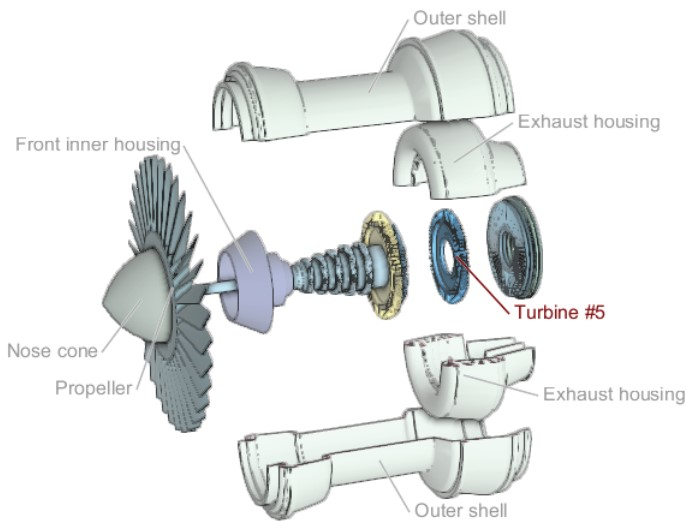
\includegraphics[width=.95\linewidth]{fig/Images/AutomatedGenerationofInteractive3DExplodedViewDiagrams_Li2008_fig1}
		\caption[]{System presented by Li et al.[\cite{Wilmot_Li_2008}, Figure 1]}
		
	\end{subfigure}
	\smallskip
	\begin{subfigure}[t]{0.5\textwidth}
		\centering
		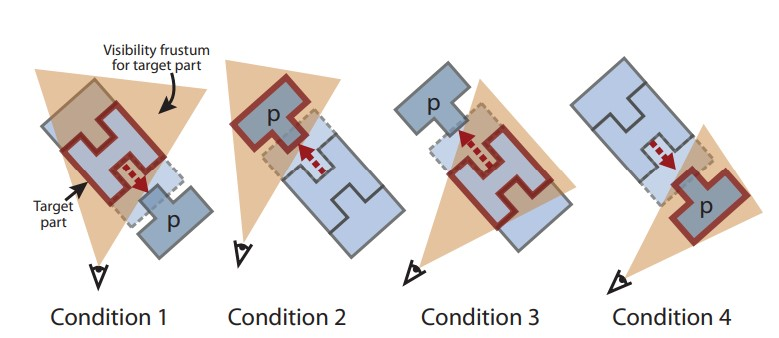
\includegraphics[width=1.1\linewidth]{fig/Images/AutomatedGenerationofInteractive3DExplodedViewDiagrams_Li2008_fig8}
		\caption[]{Conditions for moving part $p$. For each condition, the target part is outlined in red. The orange visibility frusta show how unwanted occlusions have been eliminated in each case. [\cite{Wilmot_Li_2008}, Figure 8]}
	\end{subfigure}
\end{figure}
The algorithm works by calculating an explosion graph when loading the model, which describes the blocking elements of each part from different angles. 
This allows to retrieve at runtime the sequence of elements needed to disassemble the object without parts passing through others. 
Thus a dynamic explosion graph can be generated which shows an animated composition from all viewing directions.
An important part of this is the generation of a correct explosion graph. 
To accomplish this, two problems have to be solved: first, how to move the parts to uncover the target parts without occluding them, and second, how to deal with enclosed parts. 
\begin{wrapfigure}{r}{0.25\textwidth}
	\centering
	\vspace{-0.4cm}
	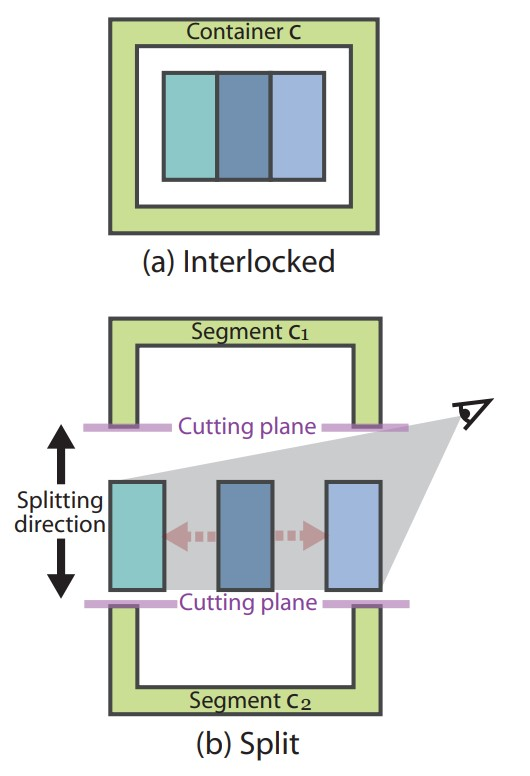
\includegraphics[width=1\linewidth]{fig/Images/AutomatedGenerationofInteractive3DExplodedViewDiagrams_Li2008_fig7}
	\caption[]{Splitting container to reveal enclosed parts [\cite{Wilmot_Li_2008}, Figure 7]}
	\vspace{-0.8cm}
\end{wrapfigure}
Li et al. solve this problem by iteratively going through all the parts and testing for two conditions: each part must be moved so that none of the target parts are obscured; if the part is a target part, it must not be obscured by any part that has already been visited. 
In order to isolate target parts from other touching parts, it is also made sure that they are completely visible and close parts are moved further away. 
If one part is completely enclosed by another, the outer one is separated in the bounding box center and pulled apart so that the inner parts are completely visible, then the algorithm continues.
The resulting application generates animated exploded views for models with up to fifty parts. 
However, a disadvantage of this implementation is that it only works for static data sets and does not provide any solution for time-varying data sets.

Tatzgern et al. improve on the work of Li et al. by finding frequently recurring subsets in a mesh and grouping them, then selecting the best representative of that group and exploding it based on a quality score.\cite{Tatzgern_2010}
The frequently recurring subsets are found automatically based on a frequent sub-graph search. %TODO add pictures
The resulting explosion diagrams are especially useful for technological models where there are many identical subsets, and the explosion displays only one of them instead of doing this for each of these subsets and taking up a lot of screen space.  
For biological datasets, however, this extension is less useful, since it brings little advantage due to the distinct structure of biological objects.
More relevant, however, is its quality score which is used to select the representative. This is also applicable to general explosion views and can be used to quantitatively describe the quality of an explosion view. It is defined by the following evaluation criteria: 


\begin{itemize}
	\item \textbf{Size of the footprint of the exploded view:} Describes the entire screen space that the exploded view occupies.
	\item \textbf{Visibility of parts of the exploded group:} Describes the relative measure for the general visibility of the parts.
	\item \textbf{Part directions relative to current camera viewpoint:} Assumes that explosions similar to viewing direction are more difficult to read, they compute the average dot product between the viewing angle and the explosion direction.
	\item \textbf{Size of footprint of all other similar groups without any displacements:} Describes how well other similar groups are visible when selected representative is exploded.
\end{itemize}

These criteria are then weighted by Tatzgern et al., which influences the selection of the representative.
Even if not all of these points are suitable for use in virtual reality, some ideas can still be applied. In particular, using the dot product between the camera position and the direction of the exploding parts is a helpful approach.

While Li et al. and Tatzgern et al. relied on calculating the position of the exploded parts, Bruckner et al. used various \textbf{force-based techniques} to transform parts to generate explosion diagrams.\cite{Bruckner_2006}
Their presented method works with volumetric data sets and splits them into pieces before exploding them. 
For this purpose, they present three tools that interactively split the dataset at runtime using split axes and cutting planes. 
The first tool splits the first object hit by a ray based on the camera's viewing direction, the second splits all objects not just the first, while the third allows the user to draw a line onto which all parts are projected, if the projection lies on the line the part is split. 
These tools are designed to work with volumetric data sets and can also be applied to voxel data sets and are therefore suitable for biological objects.
Another interesting approach they use is the definition of forces acting on all parts to explode the object.
These forces are defined by Bruckner et al. as follows:

\begin{itemize}
	\item \textbf{Return force:} The part should move as little as possible from its original position. Therefore, there is a force pushing the part back to its original position. Bruckner et al use the following formula, where $r$ is the vector from the current vertex position to that of its original and $c_r$ is a constant factor. 
	\begin{equation}
		F_r = c_r * ln(\|r\|) * \frac{r}{\|r\|}
		\label{eq:returnforce}
	\end{equation}
	
	\item \textbf{Explosion force:} The user can select individual parts and the force will push all other parts away from the selected parts. Bruckner et al. use the following formula to describe the force $F_e$ that emanates from each selected part and acts on every part $P_i$.
	\begin{equation}
		F_e = \frac{c_e}{e^{\|r\|}} * \frac{r}{\|r\|}
		\label{eq:explosionforce}
	\end{equation}
	Here $c_e$ is a constant factor and $r$ is a vector from the explosion point to the closest point of the geometry of part $P_i$.

	\item \textbf{Viewing force:} To make the exploded view interactive, Bruckner et al. introduce another force that takes the camera position into account, obscuring parts are thus pushed away from the viewing direction. The procedure is described by Bruckner et al. as follows: 
	"For a part $P_i$ we determine the point along the viewing ray corresponding to the explosion point’s projection which is closest to
	the center of $P_i$. The force $Fv$ is then:"
	\begin{equation}
		F_v = \frac{c_v}{\|r\|} * \frac{r}{\|r\|}
		\label{eq:viewingforce}
	\end{equation}
	Here $c_v$ is again a constant factor and $r$ a vector which points from the shortest point on the viewing axis to the center of the part $P_i$.  

	\item \textbf{Spacing force:} The last force $F_s$ pushes all parts away from each other to avoid overlapping and is described by the following formula:
	\begin{equation}
		F_v = \frac{c_s}{\|r\|^2} * \frac{r}{\|r\|}
		\label{eq:spacingforce}
	\end{equation}
	Again, $c_s$ is a constant factor and $r$ is a vector pointing from the center of part $P_i$ to the center $P_j$ of every other part.
\end{itemize}

These forces are then weighted by Bruckner et al. and applied to each part.
\begin{figure}[t]
	\centering
	%\vspace{-0.7cm}
	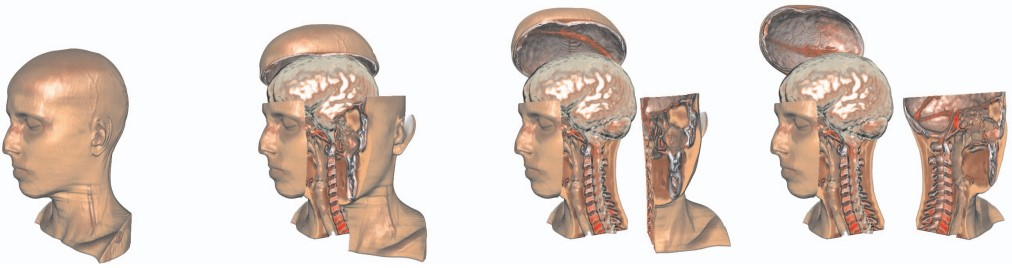
\includegraphics[width=.95\linewidth]{fig/Images/Bruckner_fig2}
	\caption[]{Interactive exploded-view illustration of a human head with increasing degrees-of-explosion created by Bruckner et al. using their force-based approach. [\cite{Bruckner_2006}, Figure 2]}
\end{figure}
The result is a view-dependent explosion diagram which can be edited and expanded at runtime. 
Thus, it is also possible to uncover enclosed parts by separating the outer part through user input.

Sonnet et al. also use a similar force-based approach.\cite{Sonnet_2004}
However, their application differs in that a probe is used for explosion which the user can move through the dataset and whose effect radius determines the translation of the parts. 
An interesting addition presented for dealing with enclosed objects is that when loading the data set, the size of the bounding box determines the weight of the object. 
Smaller objects that are inside a larger one will hence be pushed away stronger from the effect radius of the probe. 
This method is a simple way to avoid occlusion in the case of an enclosed object, but it causes problems when the point used to explode the inner and outer object are the same, since the weighting then has no influence.

\textbf{Virtual reality} opens up new possibilities to interact with and study exploded views. In their paper, He et al. describe several types of interaction methods to explore a CAD model of a brain using VR devices.\cite{He2017}
To compute an explosion graph that defines the transformation of the parts, they use the bounding box of each mesh, then build a complete bounding volume hierarchy from the bottom-up.
This is necessary because medical data does not have a specific assembly order that can be revealed. 
In their work, they use parent-child relationships to constrain the transformation and guide it in a constructive manner.
To allow for easy manipulation of the exploded view's axis, they use Hermit splines, which can be drawn with VR controllers. They also describe several ways of interacting with the mesh to trigger different exploded views:

\begin{itemize}
	\item \textbf{linear explosion:} The user defines an axis by moving the controllers apart in parallel, the mesh is then pulled apart along this axis.
	\item \textbf{leafing interaction:} He et al. describe this interaction as slicing the object and then leafing through the pieces as if one were leafing through a book.
	\item \textbf{fanning interaction:} This interaction also first cuts the object into slices, then the individual slices are fanned out as if you were holding playing cards with their backs facing upwards in front of you. 
\end{itemize}

%TODO add pictures
Not only the interaction with VR plays an important role in this work, but also the special feature of a \textbf{time-varying data set}. 
Special measures are necessary to display these in an exploded view, but after extensive research no related work could be found. 
Therefore, in this work, a focus must be placed on solving this problem.

While exploded views are a large part of this work, they are not the only way to avoid occlusion. 
Another approach that can be combined well with interaction in VR is the use of \textbf{magic lenses}.
This is like a kind of magnifying glass that allows the user to look inside an object and hide the obscuring geometry of the surface.
One advantage of this over cutting planes is that the context is preserved because only a selective subarea is hidden.   
One possible implementation of this has been described by Viega et al. among others.\cite{Viega_1996}
They hide the surface of a hand to reveal the underlying skeleton. %TODO add pictures
The same concept was extended by Hua et al. to work in augmented reality with a physical prototype.\cite{Hua_2006}
This also works like a magnifying glass which can be moved over a desktop and thus enables a look into the interior of various objects. 
For example, you can look inside the buildings of a model of a city or explore the inside of a human body.
Their user study showed that "magic lenses are efficient cognitive filters that dynamically organize and display data when and where it is needed."\cite{Hua_2006}
They proved to be more efficient and intuitive than a traditional interface, although their prototype lacked stability.
Another alternative approach, which is combinable, is proposed by Preim et al. In their paper, they use different scaling techniques to enlarge and dynamically label objects of interest, making it easier to identify details.\cite{Preim_1997}

Another unique method was presented by McGuffin et al.\cite{McGuffin}
They show various tools they have developed to inspect volumetric data by peeling and cutting parts away.
They introduce a Leafer tool to slice and open the dataset, and a Peeler tool to show different layers of the dataset. They also introduce a Boxspreader tool that pushes voxels away, a Hinge Spreader tool, and a Sphere Extender tool to cut and extend different layers of the dataset.
With these, complex transformations of the data are possible, which can provide insights into the interior of various volumetric data sets.
One observation made by McGuffin et al. is that animations have greatly improved the usability of these tools, because without them, users had difficulty understanding how the tools operated. 

Another related work was presented by Tania Krisanty at the Chair of Computer Graphics at the TU Dresden. She uses a similar slightly simplified version of the same data set used in this work and shows the use of cutting planes in virtual reality.\cite{krisanty_2022}
She presents several interactions in virtual reality, like grabbing a new cutting plane from an imaginary backpack. 
One problem that arises is the loss of context when viewing the inner cells, a possibility that has been developed for this is the selective deactivation of cells, which eases the examination of individual cells in the interior, but does not solve the problem completely.

